\documentclass[../main.tex]{subfiles}
\begin{document}
\captionsetup[figure]{labelfont={bf},name={FIGURE},labelsep=period, justification = raggedright, singlelinecheck = false}

\chapter{Determinants} \label{ch:4}
\noindent\textit{You should be familiar with}
\begin{itemize}[leftmargin=*]
  \setlength{\itemsep}{0pt}
  \setlength{\parskip}{0pt}
  \item Matrix row elimination
  \item Linear systems of equations
\end{itemize}
The determinant is defined for any \(n \times n\) matrix and produces a scalar value. You have propably dealt with determinants before, possibly while using Cramer's rule. The determinant has many theoretical uses in linear algebra. Among these is the definition of eigenvalues and eigenvectors, as we will see in Chapter.~\ref{ch:5}. In Section~\ref{sec:det_devel}, we will develop a formula for the inverse of a matrix of all first-order partial derivatives of a multivariate function. The determinant of the Jacobian matrix, called the Jacobian, is used in multivariable calculus.

Although the determinant has theoretical uses, because of the complexity of its calculation, a determinant is seldom used in practice unless the matrix size is small. In this chapter, we will begin with the definitions of the determinant and then discuss its evaluation using expansion by minors and Gaussian elimination. This chapter ends with an interesting example where determinants play a role in file encryption. \\


\section{Developing the determinant of a \(2 \times 2 \) and a \(3 \times 3\) matrix} \label{sec:det_devel}
\noindent{}The determinant of an \(n \times n\) matrix is the sum of all possible products of n elements formed by choosing one element from each row in order \(1, 2, \cdots, n\) in different collumns along with the proper sign. The sign is found by writing down the sequence of column indices in each product and counting the number of interchanges necessary to put the column indices in the order \(1, 2, \cdots, n\). If the number of interchanges is even, then the sign is \(+\); otherwise, the sign is \(-\).

\begin{example} \label{ex:two_det} Find the determinant of the general \(2 \times 2\) matrix \(A = 
  \begin{bmatrix}
  a_{11} & a_{12} \\
  a_{21} & a_{22} 
  \end{bmatrix} 
  \).
  First list the products without the sign. Note that in the first product, we choose \(a_{11}\) from row \(1\) and \(a_{22}\) from row \(2\). In the second product, we choose \(a_{12}\) from row \(1\) and \(a_{21}\) from row \(2\).
  
\(a_{11}a_{22}	a_{12}a_{21}\)

In the first product, the sequence if column indices is \(1, 2\), so its sign is \(+\). In the second product, the column indices are in the order \(2, 1\), so its sign is \(-\). Thus, the determinant of \(A, det(A)\), is \[det(A) = a_{11}a_{22} - a_{12}a_{21}.\]
\end{example}

Example \ref{ex:two_det} finds the formula for the determinant of a \(3 \times 3\) matrix. After reading trough the example, you will see why we will not give the formula fo the determinant of a \(4 \times 4\) matrix.

\begin{example} \label{ex:three_det} Let \(A = 
  \begin{bmatrix}
  a_{11} & a_{12} & a_{13} \\
  a_{21} & a_{22} & a_{23} \\
  a_{31} & a_{32} & a_{33} 
  \end{bmatrix}
  \). Here is the sum of products, each with its sign.
  \begin{equation*}
    \begin{aligned}
      &a_{11}a_{22}a_{33} - a_{11}a_{23}a_{32} - a_{12}a_{21}a_{33} + a_{12}a_{23}a_{31} + a_{13}a_{21}a_{32} - a_{13}a_{22}a_{31} = \\ 
      &a_{11}(a_{22}a_{23} - a_{23}a_{32}) - a_{12}(a_{21}a_{33} - a_{23}a_{31}) + a_{13}(a_{21}a_{32} - a_{22}a_{31})
    \end{aligned}  
  \end{equation*}
\end{example}
  Note that the number of products to be evaluated in a \(2 \times 2\) matrix is \(2 = 2(1) = 2!\), and in \(3 \times 3\) matrix is \(6 = 3(2)(1) = 3!\). In general, to evaluate the determinant of an \(n \times n\) matrix involves choosing one of \(n\) elements in row \(1\), then one of \((n - 1)\) elements in row \(2, \cdots\), and \(1\) element in row \(n\), for a total of \(n(n-1)(n-2)\cdots(2)(1) = n!\) products. For instance, to evaluate the determinant of a \(15 \times 15\) matrix, requires computation of \(15! = 1,307,674,368,000\) products. This is an unbeliebably huge number of products, and it would be futile to try to use the definition of a determinant even with a supercomputer.
  
\begin{remark} \label{rm:other_det} 

Another and sometimes more convenient notation for the determinant of a square matrix \(A\) is \(|A|\).
\end{remark}

Using the definition is "messy", but from Examples \ref{ex:two_det} and \ref{ex:three_det}, we can introduce the concept of evaluating a determinant using expansion by minors. Looking at the result of example \ref{ex:three_det}, each factor in parentheses is the determinant of a \(2 \times 2\) matrix by the result of Example \ref{ex:three_det}. Thus, the determinant of \(3 \times 3\) matrix 
\(A = 
  \begin{bmatrix}
  a_{11} & a_{12} & a_{13} \\
  a_{21} & a_{22} & a_{23} \\
  a_{31} & a_{32} & a_{33} 
  \end{bmatrix}
\)
 has the value
 \begin{equation} \label{eq:three_minor}
   a_{11}
   \begin{vmatrix}
     a_{22} & a_{23} \\
     a_{32} & a_{33}
   \end{vmatrix}
   -a_{12}
   \begin{vmatrix}
     a_{21} & a_{23} \\
     a_{31} & a_{33} 
   \end{vmatrix}
   +a_{13}
   \begin{vmatrix}
     a_{21} & a_{22} \\
     a_{31} & a_{32} 
   \end{vmatrix}
 \end{equation}
  
\noindent Looking at Equation \ref{eq:three_minor}, note that the multipliers of the determinants move trough row \(1\) in the order column \(1, 2\) and \(3\) and alternate in sign. Each term contains the determinant of \(2 \times 2\) matrix obtained by crossing out the row and column of the multiplier. This process can be generalized to what is termed \textit{expansion by minors.}

\section{Expansion by minors} \label{sec:minor_exp}
\noindent In Section \ref{sec:det_devel}, we found a formula for the determinant of a \(2 \times 2\) and a \(3 \times 3\) matrix and indicated that those results can be generalized to compute the determinant of an \(n \times n\) matrix. This process, stated in Theorem \ref{th:4_1} without proof, is said to be \textit{recursive} because it involves computing determinants of smaller matrices until the problem reduces to evaluating determinants of \(2 \times 2\) matrices.

\begin{theorem} \label{th:4_1}
  Let \(M_{ij}(A)\)(or simply \(M_{ij}\), if there is no ambiguity) denote the determinant of the \((n-1) \times (n-1)\) submatrix od \(A\) formed by deleting the \(ith\) row and \(jth\) column of \(A\). Assume that the determinant function has been defined for matrices of size \((n-1) \times (n-1)\). Then the determinant of the \(n \times n\) matrix \(A\) is defined by what we call the first-row Laplace expansion: 
  \begin{equation*}
    \begin{aligned}
      |A| &= a_{11}M_{11}(A)-a_{12}M_{12}(A) + \cdots + (-1)^{1+n}M_{1n}(A) \\
          &= \sum^{n}_{j=1}(-1)^{1+j}a_{1j}M_{1j}
    \end{aligned}
  \end{equation*}
  The values \(M_{ij}\) are termed minors, and the evaluation process in Theorem \ref{th:4_1} is an example of expansion by minors.
\end{theorem}

\begin{example} \label{ex:4_3}
  Compute the \(3 \times 3\) matrix \(
  \begin{bmatrix}
    1 & 2 & −1 \\
    0 & 4 & 1 \\
    3 & 5 & −9 
  \end{bmatrix}
  \).
  \begin{equation*}
    \begin{aligned}
      \begin{vmatrix}
        1 & 2 & −1 \\
        0 & 4 & 1 \\
        3 & 5 & −9 
      \end{vmatrix}
      &= (1)
      \begin{vmatrix}
        4 & 1 \\
        5 & -9 
      \end{vmatrix}
      -(2)
      \begin{vmatrix}
        0 & 1 \\
        3 & -9 
      \end{vmatrix}
      +(-1)
      \begin{vmatrix}
        0 & 4 \\
        3 & 5 
      \end{vmatrix}\\
      &= (1)(-41)-(2)(-3)+(-1)(-12) = -23 
    \end{aligned}
  \end{equation*}
\end{example}

\begin{example} \label{ex:4_4}
  A matrix and its transpose have equal determinants; that is \(|A^T| = |A|\) (Problem \ref{pr:4_19}).
  \begin{equation*}
    \begin{aligned}
      \begin{vmatrix}
        1 & 0 & 2 \\
        1 & 2 & 2 \\
        3 & -1 & 1 
      \end{vmatrix}
      &=(1)
      \begin{vmatrix}
        2 & 5 \\
        -1 & 1 
      \end{vmatrix}
      -(0)
      \begin{vmatrix}
        1 & 5 \\
        3 & 1 
      \end{vmatrix}
      +(2)
      \begin{vmatrix}
        1 & 2 \\
        3 & -1 
      \end{vmatrix}
      = 7-14 = -7
      \\
      \begin{vmatrix}
        1 & 1 & 3 \\
        0 & 2 & -1 \\
        2 & 5 & 1 
      \end{vmatrix}
      &=(1)
      \begin{vmatrix}
        2 & -1 \\
        5 & 1 
      \end{vmatrix}
      -(1)
      \begin{vmatrix}
        0 & -1 \\
        2 & 1 
      \end{vmatrix}
      +(3)
      \begin{vmatrix}
        0 & 2 \\
        2 & 5 
      \end{vmatrix}
      = 7-2-12 = -7
    \end{aligned}
  \end{equation*}
  Sometimes the calculation of the determinant by minors (generally a tedious process) is simple.
\end{example}

\begin{theorem} \label{th:4_2}
  If a row of a matrix is zero, then the value of the determinant is 0.
  \begin{proof}
  	Assume the matrix has the form
  	\(\begin{bmatrix}
  	  a_{11} & a_{12} & a_{13} & \hdots & a_{1,n-1} & a_{1n}\\
  	  a_{21} & a_{22} & a_{23} & \hdots & a_{2,n-1} & a_{2n}\\
  	  \vdots & \vdots & \ddots & \hdots & \hdots & \vdots\\
  	  0 & 0 & 0 & \hdots & \hdots & 0\\
  	  a_{n1} & a_{n2} & a_{n3} & \hdots & \hdots & a_{nn}\\
  	\end{bmatrix}\).
  	When we expand by minors across the first row, each \((n-1) \times (n-1)\) matrix has a row of zeros. This continues as we proceed with ever smaller matrices. Finally, we will arrive at a set of \(2 \times 2\) matrices each with a row of zeros, and such a matrix has a determinant of 0.
  \end{proof}
\end{theorem}

\begin{example}
  Let \(A =
    \begin{bmatrix}
	  1 & -1 & 6\\
	  0 & 0 & 0\\
	  -8 & 9 & 10
    \end{bmatrix}	    
  \).
  \begin{equation*}
    \begin{vmatrix}
	  1 & -1 & 6\\
	  0 & 0 & 0\\
	  -8 & 9 & 10
    \end{vmatrix}
    =(1)
    \begin{vmatrix}
	  0 & 0\\
	  9 & 10
    \end{vmatrix}
    -(-1)
    \begin{vmatrix}
	  0 & 0\\
	  -8 & 10
    \end{vmatrix}
    +(6)
    \begin{vmatrix}
	  0 & 0\\
	  -8 & 9
    \end{vmatrix}
    =0
  \end{equation*}
\end{example}

Another determinant it is easy to evaluate is that of a lower triangular matrix.
\begin{equation*}
  \begin{vmatrix}
    a_{11} & 0 & \hdots & 0\\
	a_{21} & a_{22} & \hdots & 0\\
	\vdots & \vdots & \ddots & \\
	a_{n1} & a_{n2} & \hdots & a_{nn}
  \end{vmatrix}
\end{equation*}
Its determinant is the product of the diagonal elements, \(a_{11}a_{22} \hdots a_{nn}\). We can observe this by observing the sequence of expansion by minors.
\begin{equation*}
  \begin{vmatrix}
    a_{11} & 0 & \hdots & 0\\
	a_{21} & a_{22} & \hdots & 0\\
	\vdots & \vdots & \ddots & \\
	a_{n1} & a_{n2} & \hdots & a_{nn}
  \end{vmatrix}
  =a_{11}
  \begin{vmatrix}
    a_{22} & 0 & \hdots & 0\\
	a_{32} & a_{33} & \hdots & 0\\
	\vdots & \vdots & \ddots & \\
	a_{n2} & a_{n3} & \hdots & a_{nn}
  \end{vmatrix}
  =a_{11}a_{22}
  \begin{vmatrix}
    a_{33} & 0 & \hdots & 0\\
	a_{43} & a_{44} & \hdots & 0\\
	\vdots & \vdots & \ddots & \\
	a_{n3} & a_{n4} & \hdots & a_{nn}
  \end{vmatrix}
  =\cdots
\end{equation*}
We continue this process until evaluating \(2 \times 2\) matrix. At this point, we are done and have computed the value \(a_{11}a_{22} \hdots a_{nn}\)

We will leave it to exercises, but the same result applies to the determinantt of an \emph{upper triangular matrix}.\[|A| = a_{11}a_{22} \hdots a_{nn}.\]
A special case that plays a role in applications is when A is a diagonal matrix. If
\begin{equation*}
  A = diag(a_{11}, \hdots, a){nn}) = 
  \begin{bmatrix}
    a_{11} &\\
    & a_{22} &\\
    & & \ddots &\\
    & & & a_{n-1,n-1} &\\
    & & & & a_{nn}
  \end{bmatrix},
\end{equation*}
then \(|A| = a_{11} \hdots a_{nn}\). In particular, for a scalar matrix product \(tI\), we have \(det(tI) = t^n\).
\begin{remark}
  A very useful fact concerning determinants is that \(det(AB) = det(A)det(B)\). We will not provide a proof, bot will use this result numerous times.
\end{remark}
\begin{example}
  Let \(A = 
    \begin{bmatrix}
	  1 & 4 & 5\\
	  0 & -9 & 12\\
	  0 & 0 & 2
    \end{bmatrix}
  \) and \(B=
    \begin{bmatrix}
	  8 & 0 & 0\\
	  100 & 2 & 0\\
	  2 & 6 & -1
    \end{bmatrix}
  \). Note that \(A\) is upper triangular and \(B\) is lower triangular, so
  \[|A||B| = [(1)(-9)(2)][(8)(2)(-1)] = 288.\]
  The matrix \(AB\) is 
  \begin{equation*}
    AB =     
    \begin{bmatrix}
      418 & 38 & -5\\
      -876 & 54 & -12\\
      4 & 12 & -2
    \end{bmatrix}.
  \end{equation*}
  This determinant would be a chore to evaluate using expansion by minors, so we will use the MATLAB function \texttt{det.}
  \begin{lstlisting}[numbers=none,frame=none]
    >>det(C)
    
    ans = 
      288.0000
  \end{lstlisting}
\end{example}
The evaluation of an \(n \times n\) matrix was presented in terms of the first-row expansion. Actually, we can expand the determinant along any row or column, and we call this \emph{expansion by minors}.
\begin{equation*}
  det A = \sum^n_{j=1}(-1)^{i+j}a_{ij}M_{ij}(A)
\end{equation*}
is the \(i\)th row expansion and 
\begin{equation*}
  det A = \sum^n_{i=1}(-1)^{i+j}a_{ij}M_{ij}(A)
\end{equation*}
is the \(j\)th row expansion.
\begin{remark}
  The expression \((-1)^{i+j}\) obeys the chessboard pattern of signs:
  \begin{equation*}
    \begin{bmatrix}
      + & - & + & \cdots\\
      - & + & - & \cdots\\
      + & - & + & \cdots\\
      \vdots
    \end{bmatrix}
  \end{equation*}
\end{remark}

\begin{example}
  Evaluate \(
  \begin{vmatrix}
    1 & 1 & -1\\
    2 & 0 & 3\\
    8 & -7 & 1
  \end{vmatrix}
  \) using expansion by minors across row 2.
  \begin{equation*}
    \begin{vmatrix}
      1 & 1 & -1\\
      2 & 0 & 3\\
      8 & -7 & 1
    \end{vmatrix}
    =-(2)
    \begin{vmatrix}
      1 & -1\\
      -7 & 1
   \end{vmatrix}
   +(0)
    \begin{vmatrix}
      1 & -1\\
      8 & 1
   \end{vmatrix}
   -(3)
    \begin{vmatrix}
      1 & 1\\
      8 & -7
   \end{vmatrix} = 12 + 0 + 45 = 57.
  \end{equation*}
  Using the Laplace expansion, we get
  \begin{equation*}
    \begin{vmatrix}
      1 & 1 & -1\\
      2 & 0 & 3\\
      8 & -7 & 1
    \end{vmatrix}
    =(1)
    \begin{vmatrix}
      0 & 3\\
      -7 & 1
   \end{vmatrix}
   -(1)
    \begin{vmatrix}
      2 & 3\\
      8 & 1
   \end{vmatrix}
   +(-1)
    \begin{vmatrix}
      2 & 0\\
      8 & -7
   \end{vmatrix} = 12 + 0 + 45 = 57.
  \end{equation*}
\end{example}

As we have said, the determinant is primarily a theoretical tool, and one matrix built by using determinant is useful in that regard.

\begin{definition}[Cofactor]
The \((i,j)\) cofactor of \(A\), denoted by \(C_{ij}(A)\)(or \(C_{ij}\) if there is no ambiguity), is defined by \[C_{ij}(A) = (-1)^{i+j}M_{ij}(A).\]
\end{definition}
\begin{remark}
  Notice that \(C_{ij}(A)\), like \(M_{ij}(A)\), does not depend on \(a_{ij}\).
\end{remark}

\begin{definition}[Adjoint] \label{def:4_2}
  If \(A = [a_{ij}]\) is an \(n \times n\) matrix, the \emph{adjoint of A}, denoted by \(adj A\), is the transpose of the matrix of cofactors. Hence,
  \begin{equation*}
    \begin{bmatrix}
      C_{11} & C_{21} & \hdots & C_{n1}\\
      C_{12} & C_{22} & \hdots & C_{n2}\\
      \vdots &  &  & \vdots\\
      C_{1n} & C_{2n} & \hdots & C_{nn}
    \end{bmatrix}
  \end{equation*}
\end{definition}

\begin{example} \label{ex:4_8}
  Let \(A = 
  \begin{bmatrix}
    1 & 2 & 3\\
    4 & 5 & 6\\
    7 & 8 & 9
  \end{bmatrix}\).
  \begin{equation*}
    \begin{aligned}
      adj(A) &= 
      \begin{bmatrix}
        C_{11} & C_{21} & C_{31}\\
        C_{12} & C_{22} & C_{32}\\
        C_{13} & C_{23} & C_{33}
      \end{bmatrix}\\
      &=\begin{bmatrix}
          \begin{vmatrix}
            5 & 6\\
            8 & 9
          \end{vmatrix}
          &-\begin{vmatrix}
            2 & 3\\
            8 & 9
          \end{vmatrix}
          &\begin{vmatrix}
            2 & 3\\
            8 & 9
          \end{vmatrix}\\
          
          -\begin{vmatrix}
            4 & 6\\
            8 & 9
          \end{vmatrix}
          &\begin{vmatrix}
            1 & 3\\
            8 & 9
          \end{vmatrix}
          &-\begin{vmatrix}
            1 & 3\\
            4 & 9
          \end{vmatrix}\\
          
          \begin{vmatrix}
            4 & 5\\
            8 & 8
          \end{vmatrix}
          &-\begin{vmatrix}
            1 & 2\\
            8 & 8
          \end{vmatrix}
          &\begin{vmatrix}
            1 & 2\\
            4 & 5
          \end{vmatrix}\\
      \end{bmatrix}\\
      &=\begin{bmatrix}
        -3 & 6 & -3\\
        12 & -15 & 6\\
        -8 & 8 & -3
      \end{bmatrix}
    \end{aligned}
  \end{equation*}
  In addition, compute the product of \(A\) and its adjoint:
  \begin{equation*}
    A(adj(A)) = \begin{bmatrix}
      1 & 2 & 3\\
      4 & 5 & 6\\
      7 & 8 & 9
    \end{bmatrix}
    \begin{bmatrix}
      -3 & 6 & -3\\
      12 & -15 & 6\\
      -8 & 8 & -3
    \end{bmatrix}
    =\begin{bmatrix}
      -3 & 0 & 0\\
      0 & -3 & 0\\
      0 & 0 & -3
    \end{bmatrix}
    =-3I.
  \end{equation*}
  Also compute the determinant of A.
  \begin{equation*}
    |A| = \begin{vmatrix}
      5 & 6\\
      8 & 9
    \end{vmatrix}
    -2\begin{vmatrix}
      4 & 6\\
      8 & 9
    \end{vmatrix}
    +3\begin{vmatrix}
      4 & 5\\
      8 & 8
    \end{vmatrix}
    = -3 +24 -24 = -3.
  \end{equation*}
\end{example}

Example \ref{ex:4_8} illustrates a very interesting property of the adjoint. The product of a matrix \(A\) ad its adjoint is a diagonal matrix whose diagonal entries are \(det(A)\). We will not prove this result, but will use it to develop a formula for computing the inverse of a matrix.

\begin{theorem} \label{th:4_3}
  The inverse of a matrix is related to the adjoint by the relation
  \begin{equation} \label{eq:4_2}
    A^{-1} = \frac{1}{detA} adj(A).
  \end{equation}
  \begin{proof}
    Since \begin{equation*}
      A \times adj(A) = \begin{bmatrix}
        det A & 0 & & & 0\\
        0 & det A & & & 0\\
        & & \ddots\\
        & & & det A & \\
        0 & & & & detA
      \end{bmatrix}
    \end{equation*}
    we have \(A \times adj(A) = (det A)I\). Thus, \(A((1/det A)adj(A)) = I\), and \(A^{-1} = (1/det A) adj(A)\)
  \end{proof}
\end{theorem}

\begin{example} \label{ex:4_9}
  We computed the determinant ond the adjoint of the matrix \(A = \begin{bmatrix}
    1 & 2 & 3\\
    4 & 5 & 6\\
    7 & 8 & 9
  \end{bmatrix}\)
  in Example \ref{ex:4_8}.
  
  Equation \ref{eq:4_2} computes the inverse of \(A\).
  \begin{equation*}
    A^{-1} = -\frac{1}{3}\begin{bmatrix}
      -3 & 6 & -3\\
      12 & -15 & 6\\
      -8 & 8 & -3
    \end{bmatrix}.
  \end{equation*}
\end{example}

\section{Computing a determinant using row operations}
\noindent A determinant has properties that allow its computation without resorting to expansion by minors. Example \ref{ex:4_10} demonstrates the properties.

\begin{example} \label{ex:4_10}
  \leavevmode
  \begin{enumerate}
    \item A determinant is a linear function of each row separately.\\
    If two rows are added, with all other rows remaining the same, the determinants are added.
    \begin{equation*}
      \begin{aligned}
        \begin{vmatrix}
          2 & 3 & 4\\
          -1 & -2 & -3\\
          -4 & -3 & -4
        \end{vmatrix}
        +\begin{vmatrix}
          5 & 6 & 7\\
          -1 & -2 & -3\\
          -4 & -3 & -4
        \end{vmatrix}
        &=2+8=10\\
        \begin{vmatrix}
          2+5 & 3+6 & 4+7\\
          -1 & -2 & -3\\
          -4 & -3 & -4
        \end{vmatrix}
        &=\begin{vmatrix}
          7 & 9 & 11\\
          -1 & -2 & -3\\
          -4 & -3 & -4
        \end{vmatrix}
        =10
      \end{aligned}
    \end{equation*}
    
    If a row of \(A\) is multiplied by a scalar \(t\), then the determinant of the modified matrix \(t\) is \(det A\).
    \begin{equation*}
      \begin{vmatrix}
        1 & 4 & 0\\
        (7) & (7)5 & (7)1\\
        1 & 0 & 0
      \end{vmatrix}
      =(1)
      \begin{vmatrix}
        4 & 0\\
        35 & 7
      \end{vmatrix}
      =28 = (7)
      \begin{vmatrix}
        1 & 4 & 0\\
        2 & 5 & 1\\
        1 & 0 & 0
      \end{vmatrix}
      =(7)(4)
    \end{equation*}
    \item When two rows of a matrix are equal, the determinant is zero.
    \begin{equation*}
      \begin{vmatrix}
        1 & 0 & 1\\
        2 & 1 & 8\\
        1 & 0 & 1
      \end{vmatrix}
      =(1)
      \begin{vmatrix}
        1 & 8\\
        0 & 1
      \end{vmatrix}
      -(2)
      \begin{vmatrix}
        0 & 1\\
        0 & 1
      \end{vmatrix}
      +(1)
      \begin{vmatrix}
        0 & 1\\
        1 & 8
      \end{vmatrix}
      =1-0+(1)(-1) = 0
    \end{equation*}
    
    \item If two rows of a matrix are exchaned, the determinant changes sign.
    \begin{equation*}
      \begin{vmatrix}
        1 & 0 & 0\\
        2 & 5 & 1\\
        1 & 4 & 0
      \end{vmatrix}
      =(1)
      \begin{vmatrix}
        5 & 1\\
        4 & 0
      \end{vmatrix}
      =-4\\
      \begin{vmatrix}
        1 & 4 & 0\\
        2 & 5 & 1\\
        1 & 0 & 0
      \end{vmatrix}
      =(1)
      \begin{vmatrix}
        5 & 1\\
        0 & 0
      \end{vmatrix}
      -(4)
      \begin{vmatrix}
        2 & 1\\
        1 & 0
      \end{vmatrix}
      =4
    \end{equation*}
    
    \item If multiple of a row is subtracted from another row, the value of the determinant remains unchanged.
    \begin{equation*}
      \begin{vmatrix}
        1 & 4 & 0\\
        2 & 5 & 1\\
        1 & 0 & 0
      \end{vmatrix}
      \overrightarrow{R2 = R2-8R1}
      \begin{vmatrix}
        1 & 4 & 0\\
        -6 & -27 & 1\\
        1 & 0 & 0
      \end{vmatrix}
      =(1)
      \begin{vmatrix}
        4 & 0\\
        -27 & 1
      \end{vmatrix}
      =4
    \end{equation*}
    
  \end{enumerate}
\end{example}

Theorem \ref{th:4_4} formally states the properties demonstrated in Example \ref{ex:4_10}.
\begin{theorem} \label{th:4_4}
 \leavevmode
 \begin{enumerate}[leftmargin=*]
   \item A determinant is a linear function of each row separately.
   \item If two rows of a matrix are equal, the determinant is zero.
   \item If two rows of a matrix are interchanged, the determinant changes sign.
   \item If a multiple of a row is subtracted from another row, the value of the determinant is unchanged.
 \end{enumerate}
\end{theorem}
\begin{proof}
  \begin{enumerate}[leftmargin=*]
    \item Assume matrices \(A\) and \(B\) as follows:\\
    \(A =
      \begin{bmatrix}
        a_{11} & a_{12} & \hdots & a_{1,n-1} & a_{1n}\\
        \vdots & \ddots & \hdots & \hdots & \vdots\\
        a_{i1} & a_{i2} & \hdots & a_{i,n-1} & a_{in}\\
        \vdots & \vdots & \vdots & \vdots & \vdots\\
        a_{n1} & a_{n2} & \hdots & a_{n,n-1} & a_{nn}
      \end{bmatrix}
    \), \(B=
      \begin{bmatrix}
        a_{11} & a_{12} & \hdots & a_{1,n-1} & a_{1n}\\
        \vdots & \ddots & \hdots & \hdots & \vdots\\
        a_{i1}^{'} & a_{i2}^{'} & \hdots & a_{i,n-1}^{'} & a_{in}^{'}\\
        \vdots & \vdots & \vdots & \vdots & \vdots\\
        a_{n1} & a_{n2} & \hdots & a_{n,n-1} & a_{nn}
      \end{bmatrix}
    \).\\
    Then\\
    \(\begin{vmatrix}
      a_{11} & a_{12} & \hdots & a_{1,n-1} & a_{1n}\\
      \vdots & \ddots & \hdots & \hdots & \vdots\\
      a_{i1} + a_{i1}^{'} & a_{i2} + a_{i2}^{'} & \hdots & a_{i,n-1} + a_{i, n-1}^{'} & a_{in}+ a_{in}^{'}\\
      \vdots & \vdots & \vdots & \vdots & \vdots\\
      a_{n1} & a_{n2} & \hdots & a_{n,n-1} & a_{nn}
    \end{vmatrix}=\\    
    \sum^{n}_{k=1}(-1)^{i+k}(a_{ik} + a_{ik}^{'})M_{ik} = \sum^{n}_{k=1}(-1)^{i+k}a_{ik}M_{ik} + \sum^{n}_{k=1}(-1)^{i+k}a_{ik}^{'}M_{ik} =\\
    |A| + |B| 
    \)
    
    The proof that \(det(tA) = t det(A)\) is left to Problem \ref{pr:4_13}.
    \item See Problem \ref{4_15}.
    \item See Problem \ref{4_14}.
    \item Subtract a multiple, \(t\) of row \(j\) from row \(i\).
    \begin{equation*}
      \begin{aligned}
        &\begin{bmatrix}
          a_{11} & a_{12} & \hdots & a_{1,n-1} & a_{1n}\\
          \vdots & \ddots & \hdots & \hdots & \vdots\\
          a_{i1} + ta_{j1} & a_{i2} + ta_{j2} & \hdots & a_{i,n-1} + ta_{j, n-1} & a_{in}+ ta_{jn}\\
          \vdots & \vdots & \vdots & \vdots & \vdots\\
          a_{n1} & a_{n2} & \hdots & a_{n,n-1} & a_{nn}
        \end{bmatrix}\\
        &=\begin{bmatrix}
          a_{11} & a_{12} & \hdots & a_{1,n-1} & a_{1n}\\
          \vdots & \ddots & \hdots & \hdots & \vdots\\
          a_{i1} & a_{i2} & \hdots & a_{i,n-1} & a_{in}\\
          \vdots & \vdots & \vdots & \vdots & \vdots\\
          a_{n1} & a_{n2} & \hdots & a_{n,n-1} & a_{nn}
        \end{bmatrix}
        +\begin{bmatrix}
          a_{11} & a_{12} & \hdots & a_{1,n-1} & a_{1n}\\
          \vdots & \ddots & \hdots & \hdots & \vdots\\
          -ta_{j1} & -ta_{j2} & \hdots & -ta_{j,n-1} & -ta_{jn}\\
          \vdots & \vdots & \vdots & \vdots & \vdots\\
          a_{n1} & a_{n2} & \hdots & a_{n,n-1} & a_{nn}
        \end{bmatrix} = \text{ (property 1)}\\
         &A - t\begin{bmatrix}
           a_{11} & a_{12} & \hdots & a_{1,n-1} & a_{1n}\\
           \vdots & \ddots & \hdots & \hdots & \vdots\\
           a_{i1} & a_{i2} & \hdots & a_{i,n-1} & a_{in}\\
           \vdots & \vdots & \vdots & \vdots & \vdots\\
           a_{n1} & a_{n2} & \hdots & a_{n,n-1} & a_{nn}
         \end{bmatrix}
        = A - t \times 0 = A \text{ (properties 1 and 2)}.\\
        &\text{Property 2 applies because row } j \text{ appears twice in }\begin{bmatrix}
          a_{11} & a_{12} & \hdots & a_{1,n-1} & a_{1n}\\
          \vdots & \ddots & \hdots & \hdots & \vdots\\
          a_{j1} & a_{j2} & \hdots & a_{j,n-1} & a_{jn}\\
          \vdots & \vdots & \vdots & \vdots & \vdots\\
          a_{n1} & a_{n2} & \hdots & a_{n,n-1} & a_{nn}
        \end{bmatrix}.
      \end{aligned}\\
    \end{equation*}
    
  \end{enumerate}
\end{proof}

The properties in Theorem \ref{th:4_4}  provide a means for calculating a determinant without using expansion by minors. reduce the matrix to upper triangular form, recording any sign changes caused by row interchanges, together with any factors taken out of a row. Then compute the product of the diagonal elements. Here are some examples.

\begin{example} \label{ex:4_11}
  Evaluate the determinant
  \begin{equation*}
    \begin{vmatrix}
      1 & 2 & 3\\
      4 & 5 & 6\\
      7 & 8 & 9
    \end{vmatrix}.
  \end{equation*}
  Using row operations \(R_{2} \rightarrow R_{2} - 4R_{1}\) and \(R_{3} \rightarrow R_{3} - 8R_{1}\) gives
  \begin{equation*}
    \begin{vmatrix}
      1 & 2 & 3\\
      4 & 5 & 6\\
      7 & 8 & 9
    \end{vmatrix}
    =\begin{vmatrix}
      1 & 2 & 3\\
      0 & -3 & -6\\
      0 & -8 & -15
    \end{vmatrix}.
  \end{equation*}
  Now perform the row operation \(R_{3} \rightarrow R_{3} - \frac{8}{3}R_{2}\)
  \begin{equation*}
    \begin{vmatrix}
      1 & 2 & 3\\
      4 & 5 & 6\\
      7 & 8 & 9
    \end{vmatrix}
    =\begin{vmatrix}
      1 & 2 & 3\\
      0 & -3 & -6\\
      0 & 0 & 1
    \end{vmatrix}
    =(1)(-3)(1) = -3.
  \end{equation*}
\end{example}

\begin{example}
Evaluate the determinant \(\begin{vmatrix}
      1 & 1 & 2 & 1\\
      3 & 1 & 4 & 5\\
      7 & 6 & 1 & 2\\
      1 & 1 & 3 & 4
    \end{vmatrix}
    \).\\
    Begin by using row operations to zero-out the elements in column 1, rows 2-4.
    \begin{equation*}
      \begin{aligned}
        \begin{vmatrix}
          1 & 1 & 2 & 1\\
          3 & 1 & 4 & 5\\
          7 & 6 & 1 & 2\\
          1 & 1 & 3 & 4
        \end{vmatrix}
        &=\begin{vmatrix}
          1 & 1 & 2 & 1\\
          0 & -2 & -2 & 2\\
          0 & -1 & -13 & -5\\
          0 & 0 & 1 & 3
        \end{vmatrix}\text{ (factor }-2\text{ from row }2\text{)}\\
        &= -2\begin{vmatrix}
          1 & 1 & 2 & 1\\
          0 & 1 & 1 & -1\\
          0 & -1 & -13 & -5\\
          0 & 0 & 1 & 3
        \end{vmatrix}\text{ (add row } 2\text{ to row }3\text{)}\\
        &= -2\begin{vmatrix}
          1 & 1 & 2 & 1\\
          0 & 1 & 1 & -1\\
          0 & 0 & -12 & -6\\
          0 & 0 & 1 & 3
        \end{vmatrix}\text{ (swap rows } 3 \text{ and } 4 \text{ to put 1 on the main diagonal)}\\
        &= 2\begin{vmatrix}
          1 & 1 & 2 & 1\\
          0 & 1 & 1 & -1\\
          0 & 0 & 1 & 3\\
          0 & 0 & -12 & -6
        \end{vmatrix} (R_4 \rightarrow R_4 + 12R_3)\\
        &= 2\begin{vmatrix}
          1 & 1 & 2 & 1\\
          0 & 1 & 1 & -1\\
          0 & 0 & 1 & 3\\
          0 & 0 & 0 & 30
        \end{vmatrix} \text{ (multiply the diagonal elements)}=60.
      \end{aligned}
    \end{equation*}
    
\end{example}

In Chapter \ref{ch:12}, we will introduce the Vandermonde matrix \(V = \begin{bmatrix}
  1 & x_{1} & x_{1}^{2} & \hdots & x_{1}^{n-1}\\
  1 & x_{2} & x_{2}^{2} & \hdots & x_{2}^{n-1}\\
  1 & x_{3} & x_{3}^{2} & \hdots & x_{3}^{n-1}\\
  \vdots & \vdots & \vdots & \ddots & \vdots\\
  1 & x_{n} & x_{n}^{2} & \hdots & x_{n}^{n-1}\\
 \end{bmatrix}\)
in connection with finding a polynomial that approximates data in the least-squares sense. The determinant of the Vandermonde matrix has a simple formula, and Example \ref{ex:4_13} demonstrates this for \(3 \times 3\) matrix.

\begin{example} \label{ex:4_13}
  Find the determinant of the Vandermonte matrix \(V = \begin{bmatrix}
    1 & x_{1} & x_{1}^{2}\\
    1 & x_{2} & x_{2}^{2}\\
    1 & x_{3} & x_{3}^{2}
  \end{bmatrix}\).
  \begin{equation*}
    \begin{bmatrix}
      1 & x_{1} & x_{1}^{2}\\
      1 & x_{2} & x_{2}^{2}\\
      1 & x_{3} & x_{3}^{2}
    \end{bmatrix}
    \overrightarrow{\substack{R2 = R2 - (1)R1 \\ R3 = R3 - (1)R1}}
    \begin{bmatrix}
      1 & x_{1} & x_{1}^{2}\\
      0 & x_{2} - x_{1} & x_{2}^{2} - x_{1}^{2}\\
      0 & x_{3} - x_{1} & x_{3}^{2} - x_{1}^{2}
    \end{bmatrix}
    =\begin{bmatrix}
      1 & x_{1} & x_{1}^{2}\\
      0 & x_{2} - x_{1} & (x_{2} - x_{1})(x_{2} + x_{1})\\
      0 & x_{3} - x_{1} & (x_{3} - x_{1})(x_{3} + x_{1})
    \end{bmatrix}
  \end{equation*}
  Noting that only one entry in column 1 is nonzero, expand by minors down the first column.
  \begin{equation*}
    \begin{aligned}
      &det\begin{bmatrix}
        1 & x_{1} & x_{1}^{2}\\
        0 & x_{2} - x_{1} & (x_{2} - x_{1})(x_{2} + x_{1})\\
        0 & x_{3} - x_{1} & (x_{3} - x_{1})(x_{3} + x_{1})
      \end{bmatrix}
      =det\begin{bmatrix}
        x_{2} - x_{1} & (x_{2} - x_{1})(x_{2} + x_{1})\\
        x_{3} - x_{1} & (x_{3} - x_{1})(x_{3} + x_{1})
      \end{bmatrix}=\\
      &(x_2 - x_1)(x_3 - x_1)(x_3 + x_1) - (x_3 - x_1)(x_2 - x_1)*(x_2+x_1) = \\
      &(x_2 - x_1)(x_3 - x_1)[x_3 + x_1 - (x_2 + x_1)] = (x_2 - x_1)(x_3 - x_1)(x_3 - x_2)
    \end{aligned}
  \end{equation*}
\end{example}

During row reduction froma \(A\) to \(B\), multiplying a row by a scalar and subtracting from another row does not change the determinant, \(det B = det A\); however, a row may be multiplied by a scalar or two rows exchanged. In either of these cases, it follows that \(det B = c det A\), where \(c\neq0\). Hence, \(det B \neq 0\) if and only if \(det A \neq 0\) and \(det B = 0\) if and only if \(det A = 0\). This logic leads to a useful theoretical result.

\begin{theorem} \label{th:4_5}
\leavevmode
  \begin{enumerate}[leftmargin = *]
    \item A is nonsingular if and only if \(det A \neq 0\);
    \item A is singular if and only if \(det A = 0\)
    \item The homogeneous system \(Ax = 0\) has a nontrivial solution if and only if \(det A = 0\).
  \end{enumerate}
\end{theorem}

\begin{proof}
\leavevmode
  \begin{enumerate}[leftmargin = *]
    \item Perform a sequence of elementary row operations reducing A to B, where we intend for B to be the identity matrix. B cannot have a zero row, for otherwise the homogeneous equation \(Ax = 0\) will have a nonzero solution. Thus, the reduction must be successful, so \(B = I\), and it follows that \(det A=c\) \(det I = c \neq 0\) so \(det A \neq 0\). Since \(A^{-1} = (1/|A|)adj(A)\), \(A^{-1}\) exists, and A is nonsingular.
    \item The previous statement logically implies that "\(det A =  0\) if and only if \(A\) is singular."
    \item If \(Ax = 0\) has a nontrivial solution, then reduction to upper triangular form must produce a zero row, so \(det A = 0\). If \(Ax = 0\) has a unique solution, then after reduction to upper triangular form there can be no zeros on the diagonal, or there will be infinitely many solutions. Thus \(det A \neq 0\).
  
  \end{enumerate}
\end{proof}

\begin{example} \label{ex:4_14}
  This uses MATLAB statements to illustrate Theorem \ref{th:4_5}. Note that in addition to having a zero determinant, the nullity of \(B\) is nonzero, also indicating that \(B\) is singular.
  \begin{lstlisting}[numbers=none,frame=none]
>> A = [1 6 25; 16 32 19; 56 53 5];
>>det(A)

ans=
     -18543
     
>> A\[1 2 5]'

ans=
   0.0910
  -0.0053
   0.0376
	
>> B = [1 3 2;5 14 7;2 5 1];
>>det(B)

ans=
 -3.3307e-015
>>size(null(B),2)% compute the nullity of B

ans=
    1
>> B\[1 2 5]'
Warning: Matrix iscloseto singular or badly scaled.
       Results may be inaccurate. RCOND = 4.587698e-018.
ans=
  1.0e+016 *
	
    1.2610
   -0.5404
    0.1801
  \end{lstlisting}
  Note that in the MATLAB results, \(det B\) is very small but not zero as it would be if we did the calculation by hand. The MATLAB command \texttt{det} uses the row elimination method to compute the determinant. As you will see in Chapter \ref{ch:8}, a computer in general does not perform exact arithmetic, and small errors are made during the elimination process.
\end{example}

\begin{example} \label{ex:4_15}
  Find numbers \(a\) for which the following homogenous system has a nontrivial solution and solve the system for these values of a:
  \begin{equation*}
    \begin{aligned}
      x - 2y + 3z &= 0,\\
      ax + 3y + 2z &= 0,
      6x + y + az &= 0.
    \end{aligned}
  \end{equation*}
  The determinant of the coefficient matrix is
  \begin{equation*}
    \begin{aligned}
      \Delta &= \begin{vmatrix}
        1 & -2 & 3\\
        a & 3 & 2\\
        6 & 1 & a
      \end{vmatrix}
      =\begin{vmatrix}
        1 & -2 & 3\\
        0 & 3+2a & 2-3a\\
        0 & 13 & a-18
      \end{vmatrix}
      =\begin{vmatrix}
        3+2a & 2-3a\\
        13 & a-18
      \end{vmatrix} 
    \end{aligned}
  \end{equation*}
  after expanding by minors using the first column. The value of the determinant is then
  \begin{equation*}
    (3+2a)(a-18)-13(2-3a)=2a^2+6a-80=2(a+8)(a-5).
  \end{equation*}
  So \(\Delta = 0 \Leftrightarrow a=-8 \text{ or } a=5\) and these values of \(a\) are the only values for which the given homogenous system has a nontrivial solution.
  
  If \(a=-8\), reduction of the coefficient matrix to upper triangular form gives
  \begin{equation*}
    \begin{bmatrix}
      1 & 0 & -1\\
      0 & 1 & -2\\
      0 & 0 & 0
    \end{bmatrix},
  \end{equation*}
  and so the complete solution is \(x = z, y=2z\) with \(z\) arbitrary, and the null space is spanned by \(\begin{bmatrix}
    1 \\ 2 \\ 1
  \end{bmatrix}\).
  The case of \(a=5\) is left to the excercises.
\end{example} 

If the Symbolic Toolbox is available in your MATLAB distribution, there are many posibilities for performing symbolic manipulation with linear algebra. The following is a partial quotation from the help system for the toolbox.
\begin{quote}
\textit{
Symbolic objects are a special MATLAB\textregistered{} data type introduced bythe Symbolic Math Toolbox\texttrademark{} software. They allow you to perform mathematical operations in the MATLAB workspace analytically, without calculating numeric values. You can use symbolic objects to perform a wide variety of analytical computations:...}
\end{quote}

Example \ref{ex:4_16} shows how to solve the problem in Example \ref{ex:4_15} using the Symbolic Math Toolbox. This example is entirely optional. We will introduce a small number of additional examplex using the toolbox at various points in the book.

\begin{example} \label{ex:4_16}
  The command \texttt{syms} constructs symbolic objects, in this case \texttt{a} and \texttt{A}. The command \texttt{det} operating on a symbolic matrix does symbolic calculations. Notice that it computed the same determinant that was found in Example \ref{ex:4_15}. The command \texttt{solve} finds the solutions to \(det A = 0\). After assigning \texttt{a = -8}, the first of the two values, to locations (2,1) and (3,3), the command \texttt{null(A)} finds the null space of matrix \texttt{A}. The result is that the null space is spanned by \(\begin{bmatrix}
    1 \\ 2\\ 1
  \end{bmatrix}\),
  precisely, the result of Example \ref{ex:4_15}. The command \texttt{colspace(A)} finds a basis for the column space of \texttt{A}. There are two vectors, so the rank of \texttt{A} is 2.
  
\begin{lstlisting}[numbers=none,frame=none]
>> syms a A
>>A=[1 - 2 3;a 3 2;6 1 a]

A=
[ 1, -2, 3]
[a, 3,2]
[6, 1,a]

>>D=det(A)

D=
2*a^2 + 6*a - 80

>> vals = solve(D)

vals =
  -8
   5
   
>> A(2,1) = vals(1);
>> A(3,3) = vals(1);
>>null(A)

ans=
  1
  2
  1
  
>> colspace(A)

ans=
[  1,  0]
[  0,  1]
[ -2, -1]
\end{lstlisting}
\end{example}

\noindent To finish this section, we present and old (1750) method of solving a system of \(n\) equations in \(n\) unknowns called \emph{Cramer's rule}. It is useful for solving \(2 \times 2\) and \(3 \times 3\) systems, but otherwise is too computationally expensive to use for larger systems. It does have theoretical uses in areas of mathematics as differential equations.

\begin{theorem} \label{th:4_6}
  The system of \(n\) linear equations in \(n\) unknowns \(x_1, \hdots, x_n\)
  \begin{equation*}
    \begin{aligned}
      a_{11}x_1 + a_{12}x_2 + \cdots + a_{1n}x_n &= b_1\\
      a_{21}x_1 + a_{22}x_2 + \cdots + a_{2n}x_n &= b_2\\
      & \vdots\\
      a_{n1}x_1 + a_{n2}x_2 + \cdots + a_{nn}x_n &= b_n
    \end{aligned}
  \end{equation*}
  has a unique solution if \(\Delta = det\begin{bmatrix}
    a_{11} & a_{12} & \hdots & a_{1,n-1} & a_{1n}\\
    a_{21} & a_{22} & \hdots & a_{2,n-1} & a_{2n}\\
    \vdots & \vdots & \ddots & \vdots & \vdots\\
    a_{n-1,1} & a_{n-1,2} & \hdots & a_{n-1,n-1} & a_{n-1,n}\\
    a_{n1} & a_{n2} & \hdots & a_{n,n-1} & a_{nn}\\
  \end{bmatrix}
  \neq 0\),
  namely,
  \begin{equation*}
    x_1 = \frac{\Delta_1}{\Delta}, x_2 = \frac{\Delta_2}{\Delta}, \hdots, x_n = \frac{\Delta_n}{\Delta},
  \end{equation*}
  where \(\Delta_i\) is the determinant of the matrix formed by replacing the ith column of the coefficient matrix A by the entries \(b_1, b_2, \hdots, b_n\).

\end{theorem}
\begin{proof}
  Suppose the coefficient determinant \(\Delta \neq 0\). Then \(A^{-1}\) exists and is given by \(A^{-1} = (1/\Delta)adjA\), and the system has the unique solution
  \begin{alignat}{2}
    \begin{bmatrix}
      x_1 \\ x_2 \\ \vdots \\ x_n
    \end{bmatrix}
    &=A^{-1}\begin{bmatrix}
      b_1 \\ b_2 \\ \vdots \\ b_n
    \end{bmatrix}
    =\frac{1}{\Delta}\begin{bmatrix}
      C_{11} & C_{21} & \ldots & C_{n1}\\
      C_{12} & C_{22} & \ldots & C_{n2}\\
      \vdots & & \vdots\\
      C_{1n} & C_{2n} & \ldots & C_{nn}
    \end{bmatrix}
    \begin{bmatrix}
      b_1 \\ b_2 \\ \vdots \\ b_n
    \end{bmatrix} \label{eq:4_3}\\ 
    &=
    \frac{1}{\Delta}\begin{bmatrix}
      b_1C_{11} & b_2C_{21} & \ldots & b_nC_{n1}\\
      b_1C_{12} & b_2C_{22} & \ldots & b_nC_{n2}\\
      \vdots & & \vdots\\
      b_1C_{1n} & b_2C_{2n} & \ldots & b_nC_{nn}
    \end{bmatrix} \label{eq:4_4}       
  \end{alignat}
  Consider
  \begin{equation} \label{eq:4_5}
    \Delta_i = \begin{vmatrix}
      \ldots & a_{1, i-1} & b_1 & a_{1,i+1} & \ldots\\
      \ldots & a_{2, i-1} & b_2 & a_{2,i+1} & \ldots\\
      \vdots & \vdots & \vdots & \vdots & \vdots\\
      \vdots & \vdots & \vdots & \vdots & \vdots\\
      \ldots & a_{n, i-1} & b_n & a_{n,i+1} & \ldots
    \end{vmatrix}
  \end{equation}
  The value of \(\Delta_i\) in Equation \ref{eq:4_5} is the entry in row \(i\) in Equation \ref{eq:4_4}. Hence,
  \begin{equation*}
    \begin{bmatrix}
      x_1 \\ x_2 \\ \vdots \\ x_n
    \end{bmatrix}
    =\frac{1}{\Delta}\begin{bmatrix}
      \Delta_1 \\ \Delta_2 \\ \vdots \\ \Delta_n
    \end{bmatrix}
    =\frac{1}{\Delta}\begin{bmatrix}
      \Delta_1/\Delta \\ \Delta_2/\Delta \\ \vdots \\ \Delta_n/\Delta
    \end{bmatrix}
  \end{equation*}
\end{proof}

\begin{example} \label{ex:4_17}
  Use Cramer's rule to find the solution to the system \(\begin{bmatrix}
    1 & -1 & 5\\
    8 & 3 & 12\\
    -1 & -9 & 2\\
  \end{bmatrix}
  \begin{bmatrix}
    x_1 \\ x_2 \\ x_n
  \end{bmatrix}
  =\begin{bmatrix}
  5 \\ 3 \\ 1
  \end{bmatrix}
  \). We will perform the calculations using the MATLAB function \texttt{det} and compare the result with the solution using the operator "\textbackslash."
  \begin{lstlisting}[numbers=none,frame=none]
>>A=[1-15;8312;-1 -9 2];
>>b=[513]';
>> delta =det(A);
>> x1 = det([b A(:,2) A(:,3)])/delta

x1 =
   -2.1970

>> x2 = det([A(:,1) b A(:,3)])/delta

x2 =
    0.2414

>> x3 = det([A(:,1) A(:,2) b])/delta
x3 =
    1.4877

>> A\b

ans =
   -2.1970
    0.2414
    1.4877
  \end{lstlisting}
\end{example}

\section{APPLICATION:ENCRYPTION} \label{sec:4_4}
\noindent We begin this section with an interesting and useful result about matrices having integer entries. We are able to prove this from our work with adjoints and determinants.

\begin{theorem} \label{th:4_7}
  If an \(n \times n\) matrix \(A\) has all integer entries and \(det(A) = \pm1\), then \(A^{-1}\) exists and has all integer entries.
\end{theorem}
\begin{proof}
  We have
  \begin{equation*}
    a^{-1} = \frac{1}{detA}adjA,
  \end{equation*}
  where \(adjA\) is the adjoint od \(A\). Recall that the adjoint of a is the transpose of the matrix of cofactors of \(A\)
  \begin{equation*}
    adj(A) = \begin{bmatrix}
      C_{11} & C_{21} & \ldots & C_{n1}\\
      C_{12} & C_{22} & \ldots & C_{n2}\\
      \vdots & & \vdots\\
      C_{1n} & C_{2n} & \ldots & C_{nn}
    \end{bmatrix}
  \end{equation*}
  Each cofactor \(C_{ij}=(-1)^{i+j}M_{ij}\), where \(M_{ij}\) is the minor for the entry in row \(i\), column \(j\). In this situation, each minor is the determinant of a matrix of integer entries, so every cofactor is an integer. Since \(detA = \pm1\), it follows that \(A^{-1}\) has only integer entries.
\end{proof}

There are many ways to encrypt a message, and the use of encryption has become particularly significant in recent years (e.g., due to the explosion of financial transactions on Internet). One way to encrypt or code a message uses invertible matrices. Consider \(n \times n\) invertible matrix \(A\). Convert the message into an \(n \times m\) matrix \(B\), so that \(AB\) can be computed.
Send the message generated by \(AB\). The  receiving end will need to know \(A^{-1}\) in order to decrypt the sent message using
\begin{equation*}
  A^{-1}(AB) = B.
\end{equation*}

Keep in mind that whenever an undesired intruder finds \(A\), we must be able to change it. So we should have a mechanical way of generating simple matrices \(A\) which are invertible and have simple inverse matrices. Note that, in general, the inverse of a matrix involves fractions which are not easy to send in an electronic form. The optimal solution is to have both \(A\) and its inverse have integer entries. In fact, we can use Theorem \ref{th:4_7} to generate such a class of matrices. One practical way is to start with an upper triangular matrix with entries of \(\pm1\) on the diagonal and integer entries. Since the determinant of an upper triangular matrix is the product of its diagonal elements, such am etrix will have a determinant \(\pm1\). Now use elementary row operations to alter the matrix. Do not multiply rows with nonintegers while doing elementary row operations. Recall that adding a multiple of one row to another does not change the value of a determinant, and swaping two rows just changes the sign of the determinant. Here is an example.

\begin{example}
  Consider the matrix
  \begin{equation*}
    \begin{bmatrix}
      1 & 2 & 9\\
      0 & -1 & 3\\
      0 & 0 & 1
    \end{bmatrix}.
  \end{equation*}
  Add the first row to bot the second and third rows to obtain
  \begin{equation*}
    \begin{bmatrix}
      1 & 2 & 9\\
      1 & 1 & 12\\
      1 & 2 & 10
    \end{bmatrix}.
  \end{equation*}
  Now add the second row to the third
  \begin{equation*}
    \begin{bmatrix}
      1 & 2 & 9\\
      1 & 1 & 12\\
      2 & 3 & 22
    \end{bmatrix}.
  \end{equation*}
  Finally, add rows to and three together, multiply the sum by \(-2\) and add to the first row. We obtain the matrix
  \begin{equation*}
    A= \begin{bmatrix}
      -5 & -6 & -59\\
      1 & 1 & 12\\
      2 & 3 & 22
    \end{bmatrix}.
  \end{equation*}
  Verify that \(detA = -1\). This must be the case since the original upper triangular matrix has determinant \(-1\) and we only added multiples of one row to another.  The inverse of A is
  \begin{equation*}
    A^{-1}= \begin{bmatrix}
      14 & 45 & 13\\
      -2 & -8 & -1\\
      -1 & -3 & -1
    \end{bmatrix}.
  \end{equation*}
  Now consider the message\\
  \indent TODAY IS GOOD DAY\\
  To every letter we will associate a number. An easy way to do that is to associate \(0\) to a space, \(1\) to "A", \(2\) to "B", etc. Another way is to associate 0 to a blank or space, \(1\) to "A," \(-1\) to "B," \(2\) to "C," \(-2\) to "D," etc. Let us use the second choice. We encode our message as follows:
  \begin{table}[]
  \centering
    \begin{tabular}{|c|c|c|c|c|c|c|c|c|c|c|c|c|c|c|c|c|c|c|c|}
      \hline
      T & O & D & A & Y & & I & S & & A & & G & O & O & D & & D & A & Y\\ \hline
      -10 & 8 & -2 &  1 & 13 & 0 & 5 & 10 & 0 & 1 & 0 & 4 & 8 & 8 & -2 & 0 & -2 & 1 & 13\\ \hline
    \end{tabular}
  \end{table}
  Now we rearrange these numbers into a matrix \(B\). For example, sequence the numbers by columns, adding zeros in the last column if necessary. The matrix \(B\) must have three rows for the product \(AB\) to be defined.
  \begin{equation*}
    B = \begin{bmatrix}
      -10 & 1 & 5 & 1 & 8 & 0 & 13\\
      8 & 13 & 10 & 0 & 8 & -2 & 0\\
      -2 & 0 & 0 & 4 & -2 & 1 & 0
    \end{bmatrix}
  \end{equation*}
  Now perform the product \(AB\). We get 
\begin{equation*}
  \begin{bmatrix}
    -5 & -6 & -59\\
    1 & 1 & 12\\
    2 & 3 & 22
  \end{bmatrix}
  \begin{bmatrix}
    -10 & 1 & 5 & 1 & 8 & 0 & 13\\
    8 & 13 & 10 & 0 & 8 & -2 & 0\\
    -2 & 0 & 0 & 4 & -2 & 1 & 0
  \end{bmatrix}
  =\begin{bmatrix}
    120 & -83 & -85 & -241 & 30 & -47 & -65\\
    -26 & 14 & 15 & 49 & -8 & 10 & 13\\
    -40 & 41 & 40 & 90 & -4 & 16 & 26
  \end{bmatrix}
\end{equation*}
The encrypted message to be sent is\\
\texttt{120 -26 -40 -83 14 41 -85 15 40 -241 49 90 30 -8 -4 -47 10 16 -65 13 26}
\end{example}

\section{CHAPTER SUMMARY} \label{sec:4_5}
\subsection*{Development of the Determinant Concept}
\noindent The determinant of an \(n \times n\) matrix is a concept used primarily for theoretical purposes and it is the basis for the definition of eigenvalues, the subject of Chapters \ref{ch:5}, \ref{ch:18}, \ref{ch:19}, \ref{ch:22} and \ref{ch:23}. The original definition of a determinant is a sum of permutations with an attached sign. This definition is rarely used to evaluate a determinant. A determinant can be evaluated using a process known as expansion by minors.

\subsection*{Expansion by Minors}
\noindent Expansion by minors is a simple way to evaluate the determinant of a \(2 \times 2\) or \(3 \times 3\) matrix. For larger values of \(n\), the method is not practical, but we will see it is very useful in proving important results.

The minor, \(M_{ij}(A)\), is the determinant of the \((n-1) \times (n-1)\) submatrix of \(A\) formed by deleting the \(i\)th row and \(j\)th column of \(A\). Expansion by minors is a recursive process. The determinant of an \(n \times n\) matrix is a linear combination of the minors obtained by expansion down any row or column. By continuing this process, the problem reduces to the evaluation of \(2 \times 2\) matrices, where
\begin{equation*}
  det\begin{bmatrix}
    a_{11} & a_{12}\\
    a_{21} & a_{22}
  \end{bmatrix}
  =a_{11}a_{22} - a_{12}a_{21}.
\end{equation*}
Important properties of determinants include \begin{itemize}
  \item \(detA^T = detA\)
  \item \(det(AB) = det(A)det(B)\)
  \item If a row or column of \(A\) is zero, \(detA  = 0\).
  \item The determinant of an upper or lower triangular matrix is the product of its diagonal elements.
  \item A cofactor \(C_{ij}(A) = (-1)^{i+j}M_{ij}(A)\). The adjoint is the transpose of the matrix od cofactors, and it follows that
  \begin{equation*}
    A^{-1} = \frac{adj(A)}{detA}.
  \end{equation*}
  Like determinants in general, this result is useful for theoretical purposes. We make use of it in Section \ref{sec:4_4}.
\end{itemize}

\subsection*{Compiting a Determinant Using Row Operations}
\noindent The following facts about determinants allow the computation using elementary row operations.
\begin{itemize}
  \item If two rows are added, with all other rows remaining the same, the determinants are added, and \(det (tA) = t det(A)\) where \(t\) is a constant.
  \item If two rows of a matrix are equal, the determinant is zero.
  \item If two rows of a matrix are interchanged, the determinant changes sign.
  \item If a multiple of a row is subtracted from another row, the value of the determinant is unchanged.
\end{itemize}

Apply these rules and reduce the matrix to upper triangular form. The determinant is the product of the diagonal elements. This is how MATLAB computes \(det(A)\). As we will see in Chapter \ref{ch:8}, errors inherent in floating point arithmetic may produce an answer that is close to, but not equal to the true result.

Using row operations on a determinant, we can show that\begin{itemize}
  \item \(A\) is nonsingular if and only if \(detA \neq 0\);
  \item \(A\) is singular if and only if \(detA = 0\);
  \item The system \(Ax = 0\) has a nontrivial solution if and only if \(detA = 0\).
\end{itemize}
Although the chapter developed Cramer's rule, it should be used for theoretical use only.

\subsection*{Application of Determinants to Encryption}
Let \(A\) be an \(n \times n\) matrix. Using the result \(A^{-1} = adj(A)/detA\) the inverse of a matrix with integer entries has integer entries. Form an upper triangular matrix with integer entries, all of whose diagonal entries are \(\pm1\). Subtract integer multiples of one row from another and swap rows to "jumble up" the matrix, keeping the determinant to be \(\pm1\). Find the inverse. Encode the message as a sequence of integers stored in an \(n \times p\) matrix \(B\), and transmit \(AB\). Capture the encoded message by forming \(A^{-1}(AB) = B\).

\section{PROBLEMS}

\begin{enumerate}[label=\textbf{\thechapter.\arabic{*}}]
  \item \label{pr:4_1} Compute \(\begin{vmatrix}
    1 & -1 & 2\\
    2 & 3 & 1\\
    5 & 1 & -1
  \end{vmatrix}\)
  using the definition of a determinant as the sum over all permutations of the set \(\{1, 2, 3\}\)
  
  \item \label{pr:4_2} Using pencil and paper, evaluate the following determinants:\\
  \((a)\begin{vmatrix}
    1 & -1 & 5\\
    7 & 1 & 0\\
    3 & 3 & 3
  \end{vmatrix}\)
  \((b)\begin{vmatrix}
    -1 & 4 & 5\\
    9 & 1 & -2\\
    -4 & 1 & 3
  \end{vmatrix}\)
  
  \item \label{pr:4_3} In the matrix \(A\), an\(x\) means "any value." Show that the determinant of \(A\) is 0, regardless of the \(x\) values.
  \begin{equation*}
    A =\begin{bmatrix}
      x & x & x & x & x\\
      0 & 0 & 0 & x & x\\
      0 & 0 & 0 & x & x\\
      0 & 0 & 0 & x & x\\
      0 & 0 & 0 & x & x\\
    \end{bmatrix}.
  \end{equation*}
  
  \item \label{pr:4_4} Compute the inverse of the matrix \(A = \begin{bmatrix}
    1 & 0 & -2\\
    3 & 1 & 4\\
    5 & 2 & -3
  \end{bmatrix}\)
  by first computing the adjoint matrix.
  
  \item \label{pr:4_5} Let \(P_i = (x_i,y_i), i = 1, 2, 3\). If \(x_1, x_2, x_3\) are distinct, show that there is precisely one curve of the form \(y = ax^2 + bx + c\) passing trough \(P_1, P_2, \text{ and } P_3\).
  
  \item \label{pr:4_6} By considering the determinant and the coefficient matrix, find a relationship between \(a\) and \(b\) for which the following system has exactly one solution:\begin{equation*}
    \begin{aligned}
      x - 2y + bz &= 3,\\
      ax + 2z &= 2,\\
      5x + 2y &= 1.
    \end{aligned}
  \end{equation*}
  
  \item \label{pr:4_7} Use Cramer's rule to solve the system\\
  \(\begin{aligned}
       -2x + 3y -z &= 1\\
       x + 2y -z &= 5\\
       -2x -y +z &= -3
     \end{aligned}\)
     
  \item \label{pr:4_8} Show that\\
  \(\begin{vmatrix}
      1 & 1 & 1 & 1\\
      r & 1 & 1 & 1\\
      r & r & 1 & 1\\
      r & r & r & 1\\
    \end{vmatrix}
    =(1-r)^3
  \)
  
  \item \label{pr:4_9} Find a \(3 \times 3\) matrix consisting entirely of values \(1\) and \(-1\) that as the largest possible determinant.
  \item \label{pr:4_10} Complete Example \ref{ex:4_15} for \(a = 5\).
  \item \label{pr:4_11} Complete Example \ref{ex:4_16} for \(a = 5\).
  \item \label{pr:4_12} Prove that the determinant of an upper triangular matrix is the product of its diagonal elements.
  \item \label{pr:4_13} Prove that if a row of a square matrix \(A\) is multiplied by a scalar \(t\), then the determinant of the modified matrix is \(t det(A)\).
  \item \label{pr:4_14} In this problem, you will prove that if two rows of a matrix are interchanged, the determinant changes sign. Represent the matrix as column of rows:
  \begin{equation*}
    \begin{bmatrix}
      r_1 \\ \vdots \\ r_i \\ \vdots \\ r_j \\ \vdots \\ r_n
    \end{bmatrix}
  \end{equation*}
  By using this representation, explain the validity of each step in the proof.
  \begin{enumerate}[leftmargin=*, label=\textbf{\alph{*}.}]
    \item Add row \(j\) to row \(i\).
    \item Subtract row \(i\) from row \(j\).
    \item Add row\(j\) to row \(i\).
    \item Multiply row \(j\) by \(-1\), and the proof is complete.
  \end{enumerate}
  
  \item \label{pr:4_15} Prove that if two rows of a matrix  are equal, the determinant is zero. Hint: Exchanging the two equal rows causes the sign to change.
  \item \label{pr:4_16} Using the fact that \(|AB| = |A||B|\) show that if \(A\) is invertible, then \(|A^{-1}| = 1/|A|\).
  \item \label{pr:4_17} Show that if \(A^{T} = -A\) and \(n\) is odd, then \(|A| = 0\). Hint: \(|-A| = (-1)^n|A|\).
  \item \label{pr:4_18} Show that if \(A^2 + I = 0\), then must \(n\) be even. Hint: \(|A^2| = |A|^2\).
  \item \label{pr:4_19} Prove that \(det A = det A^T\) using mathematical induction.
  \begin{enumerate}[leftmargin=*, label=\textbf{\alph{*}.}]
    \item Show the statement is true for \(n = 2\). This is the base case.
    \item Assume the statement is true for any \(n\), and show it is true for \(n + 1\). Hint: Expansion by minors requires evaluating the determinants of \(n \times n\) matrices.
  \end{enumerate}
  
  \item \label{pr:4_20} If \(A\) is a real matrix, there is a geometrical interpretation of \(detA\) (Figure \ref{fig:1}). Let \(P = (x_1,y_1)\) and \(Q = (x_2, y_2)\) be points in the plane, forming a triangle with the origin \(O = (0,0)\).
  \begin{enumerate}[leftmargin=*, label=\textbf{\arabic{*}.}]
    \item Let \((r_1, \theta_1), (r_1, \theta_2)\) be the polar coordinate representation of \((x_1, y_1), (x_2, y_2)\), and \(\alpha = \theta_2 - \theta_1\). Show that apart from sign, \(\frac{1}{2}\begin{vmatrix}
      x_1 & y_1\\
      x_2 & y_2
    \end{vmatrix}\)
    is the area of the triangle \(OPQ\).
    
    \item Find the area of parallelogram as a determinant.
  \end{enumerate}
  \begin{figure}[h]
    \centerline{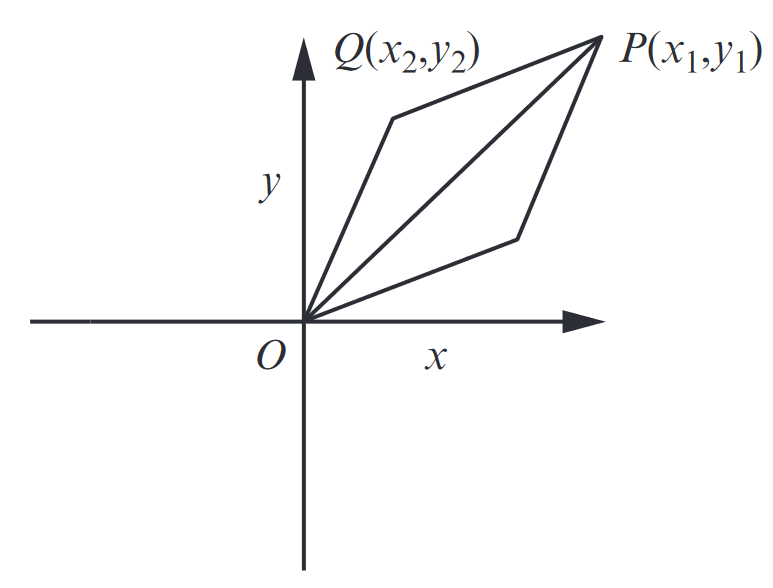
\includegraphics[scale=.3]{fig_4_1.png}}
    \caption{Geometrical interpretation of the determinant.}
    \label{fig:4_1}
  \end{figure}
\end{enumerate}

\subsection{MATLAB Problems}
\begin{enumerate}[label=\textbf{\thechapter.\arabic{*}}, resume ]
  \item \label{pr:4_21} Each matrix is singular. Verify this using the determinant, and apply the MATLAB commant \texttt{null}, to find the nullity o f each. What is the rank of \(A\) and \(B\)?\\
  \(A = \begin{bmatrix}
    1 & 19 & -122\\
    3 & 57 & -366\\
    -1 & -19 & 122
  \end{bmatrix}\), 
  \(B = \begin{bmatrix}
    1 & 0.25 & -9.25\\
    3 & 0.75 & -27.75\\
    -1 & -19 & 216.75
  \end{bmatrix}\)
  
  \item \label{pr:4_22} Evaluate the following determinants:\\
  \((a)\begin{bmatrix}
    246 & 427 & 327\\
    1014 & 543 & 443\\
    -342 & 721 & 621
  \end{bmatrix}\), 
  \((b)\begin{bmatrix}
    1 & 2 & 3 & 4\\
    -2 & 1 & -4 & 3\\
    3 & -4 & -1 & 2\\
    4 & 3 & -2 & -1
  \end{bmatrix}\).
  
  \item \label{pr:4_23} Using the Symbolic Toolbox, express the determinant of the matrix
  \begin{equation*}
    B=\begin{bmatrix}
      1 & 1 & 2 & 1\\
      1 & 2 & 3 & 4\\
      2 & 4 & 7 & 2t+6\\
      2 & 2 & 6-t & t
    \end{bmatrix}
  \end{equation*}
  as polynomial in \(t\), and determine the values of \(t\) for which \(B^{-1}\) exists.
  
  \item \label{pr:4_24} Use the Symbolic Math Toolbox to find the column space of each matrix in Problem \ref{pr:4_21}
  \item \label{pr:4_25} Use MATLAB to compute the determinant of
  \begin{equation*}
    A = \begin{bmatrix}
      20 & -34 & 8 & 12 & 3\\
      -99 & 17 & 23 & 67 & 10\\
      1 & 0 & 3 & 9 & 18\\
      3 & 5 & 0 & 9 & 11\\
      7 & 1 & 53 & 5 & 55
    \end{bmatrix}
  \end{equation*}
  
  \item \label{pr:4_26} Using MATLAB, execute\begin{lstlisting}[numbers=none,frame=none]
>> A = rosser
  \end{lstlisting}
  This creates a matrix we will use numerous times thorought the book for testing purposes.
  \begin{enumerate}[leftmargin=*, label=\textbf{\alph{*}.}]
    \item Using \texttt{rank}, verify that the matrix is singular.
    \item Compute the determinant using \texttt{det}. Is the output correct?
    \item Compute the determinant of \(A\) using Symbolic Toolbox as follows:\begin{lstlisting}[numbers=none,frame=none]
	>> syms A;
	>> A = sym(rosser);
	>> det(A)
    \end{lstlisting}
    
    \item Given the fact that MATLAB uses row operations to compute the determinant in part (b), suggest a reason for the large difference between the results of (b) and (c).
  \end{enumerate}
  
  \item \label{pr:4_27} The MATLAB command \texttt{rand(n)} builds an \(n \times n\) matrix containing pseudo random values in the range \(0 < x < 1\) drawn from the standard  uniform distribution. This means that it is equally propable you will obtain anumber from any collection of subintervals of \(0 < x < 1\) of the same length; for instance, the chance of obtaining a number from the interval \(0525 \leq x \leq 0.35\) has the same propability as obtaining a number from the interval \(0.60 \leq x \leq 0.70\). Find the determinant of random matrices of order 5, 10, 25, 50, 100, 250, 400, and 500. Doas a pattern develop? If you got \texttt{Inf} as output, what does it mean?
  
  \item \label{pr:4_28} This interesting problem was described on a MathWorks Web page. The famous Fibonacci numbers are generated from the sequence
  \begin{equation*}
    f_0 = 0,\quad f_1 = 1,\quad f_n = f_{n-1} + f_{n-2},\quad n \geq 2.
  \end{equation*}
  Most students have had some exposure to complex numbers. If not, consult Appendix \ref{app:A}. In the complex number system, the number \(i = \sqrt{-1}\), so \(i^2 = -1, i^3 = -i, i^4 = 1\), and so forth. MATLAB deals naturally with complex numbers. Create a tridiagonal matrix, with ones on the main diagonal, and \(i\) on the first sub and super diagonals with the anonymous function
  \begin{quote}
    \texttt{\footnotesize ibmat = @(n) eye(n) + diag(repmat(sqrt(-1),n-1,1),1) + diag(repmat(sqrt(-1),n-1,1),-1);}
  \end{quote}
    The command \texttt{spy(A} produces a figure placing "*" in locations that are nonzero and leaving the remainder of the figure blank. Verify that the matrix has a tridiagonal pattern by executing the following commands.\begin{lstlisting}[numbers=none,frame=none]
	>> spy(fibmat(5));
	>> figure(2);
	>> spy(fibmat(10));
	>> figure(3);
	>> spy(fibmat(25));
  \end{lstlisting}
  Compute the determinants of the sequence of matrices \texttt{fibmat(1), fibmat(2), \(\ldots\), fibmat(10)} by executing the loop\begin{lstlisting}[numbers=none,frame=none]
	for n = 1:10
		det(fibmat(n))
	end
  \end{lstlisting}
  Comment on the results.
  
  \item \label{pr:4_29} In Chapter \ref{ch:11}, we will show that if no row interchanges are performed, and \(n \times n\) matrix can be factored into a product \(A = LU\), where \(L\) is a lower triangular matrix with ones on its diagonal and \(U\) is the upper triangular matrix obtained from Gaussian elimination. For instance, if
  \begin{equation*}
    A =\begin{bmatrix}
      1 & 4 & 3\\
      2 & 9 & 12\\
      -1 & -9 & 3
    \end{bmatrix}.
  \end{equation*}
  then
  \begin{equation*}
    A =\begin{bmatrix}
      1 & 0 & 0\\
      2 & 1 & 0\\
      -1 & -5 & 1
    \end{bmatrix}
    \begin{bmatrix}
      1 & 4 & 3\\
      0 & 1 & 6\\
      0 & 0 & 36
    \end{bmatrix}.
  \end{equation*}
  \begin{enumerate}[leftmargin=*, label=\textbf{\alph{*}.}]
    \item Develop a function \\
    \texttt{function d = ludet(L,U)}\\
    that takes the factors \(L\) and \(U\) of matrix \(A\) and computes \(detA\). Check your function by computing the determinant of the matrix \(A\) using \texttt{ludet} and MATLAB's \texttt{det}.
    
    \item The function \texttt{lugauss} in the software distributuion computes the \(LU\) decomposition of a matrix without using row exchanges. It must be the case that during row elimination, a zero never appears on the diagonal. Create three matrices, of dimensions \(3 \times 3\), \(4 \times 4\), and \(5 \times 5\), and use \texttt{ludet} to compute determinant of each matrix. Verify your results using \texttt{det}.
  \end{enumerate}
  
  \item \label{pr:4_30} The \(n \times n\) Hilbert matrices are defined by \(H(i,j) = 1/(i+j-1), 1 \leq i, j \leq n\). These matrices are famous because they are ill-conditioned. A small change in a matrix entry of the right-hand side vector can cause the system \(Hx = b\) to have a very different solution. We will study ill-conditioning in Chapter \ref{ch:10}. For now, we will look at the determinants of Hilbert matrices and their inverses. The MATLAB command \texttt{hilb(n)} builds \(n \times n\) Hilbert matrix.
  \begin{enumerate}[leftmargin=*, label=\textbf{\alph{*}.}]
    \item Compute the determinant of the Hilbert matrices of order 5, 10, 15, and 25. What appears to happen as the order increases?
    \item It can be shown that the inverse of a Hilbert matrix consists entirely of integers. Compute the inverse of the Hilbert matrix of order 5.
    \item Compute the determinant of the inverse for each of the Hilbert matrices of order 5,10, 15, and 25. Relate your results to those of part (a).
  \end{enumerate}
  
  \item \label{pr:4_31} Encode the message "I LOBE LINEAR ALGEBRA" using the technique described in Section \ref{sec:4_4}. Verify that the coded message decodes correctly.
  
\end{enumerate}
\end{document}